%\documentclass[xcolor=table,handout,compress]{beamer}
\documentclass[xcolor=table]{beamer}
%--------------------------------------------------------------------------
% Common packages
%--------------------------------------------------------------------------
\usepackage[english]{babel}
\usepackage{pgfpages} % required for notes on second screen
\usepackage{graphicx}
\usepackage{subfigure}
\usepackage{multicol}
\usepackage[normalem]{ulem}

\usepackage{tabularx,ragged2e}
\usepackage{booktabs}
\usepackage{marvosym}

\makeatletter
\let\beamer@writeslidentry@miniframeson=\beamer@writeslidentry
\def\beamer@writeslidentry@miniframesoff{%
  \expandafter\beamer@ifempty\expandafter{\beamer@framestartpage}{}% does not happen normally
  {%else
    % removed \addtocontents commands
    \clearpage\beamer@notesactions%
  }
}
\newcommand*{\miniframeson}{\let\beamer@writeslidentry=\beamer@writeslidentry@miniframeson}
\newcommand*{\miniframesoff}{\let\beamer@writeslidentry=\beamer@writeslidentry@miniframesoff}
\makeatother


%--------------------------------------------------------------------------
% Load theme
%--------------------------------------------------------------------------
\usetheme{hri}

\usepackage{tikz}
\usetikzlibrary{patterns,shapes,fpu,fit,calc,mindmap,backgrounds,positioning,svg.path}

\tikzset{
  invisible/.style={opacity=0},
  visible on/.style={alt={#1{}{invisible}}},
  alt/.code args={<#1>#2#3}{%
    \alt<#1>{\pgfkeysalso{#2}}{\pgfkeysalso{#3}} % \pgfkeysalso doesn't change the path
  },
}

%% Neat trick to have only one navigation bullet per subsection
%% http://tex.stackexchange.com/questions/64333/one-navigation-bullet-per-subsection-with-subsection-false-in-custom-beamer-them
%\usepackage{etoolbox}
%\makeatletter
%\patchcmd{\slideentry}{\advance\beamer@xpos by1\relax}{}{}{}
%\def\beamer@subsectionentry#1#2#3#4#5{\advance\beamer@xpos by1\relax}%
%\makeatother
%%%%%%%%%%%%%%%%%%%%%%%%%%%%%%%%%%%%%%%

\graphicspath{{figs/}}

% for model of anthopomorphism
\newcommand{\IPA}{{$\mathcal{A}_0$~}}
\newcommand{\SLA}{{$\mathcal{A}_\infty$~}}
\newcommand{\sla}{{\mathcal{A}_\infty}}
\newcommand{\AntMax}{{$\mathcal{A}_{max}$~}}
\newcommand{\antMax}{{\mathcal{A}_{max}}}

% for HATP plans
\newcommand{\hatpaction}[3]{#1\\\textsf{\scriptsize #2,}\\\textsf{\scriptsize #3}}
\newcommand{\stmt}[1]{{\footnotesize \tt  #1}}

% for mutual modelling
\newcommand{\Mmodel}[3]{{\mathcal{M}(#1, #2, #3)}}
\newcommand{\model}[3]{{$\mathcal{M}(#1, #2, #3)$}}
\newcommand{\Model}[3]{{$\mathcal{M}^{\circ}(#1, #2, #3)$}}

% typeset logical concept
\newcommand{\concept}[1]{{\scriptsize \texttt{#1}}}

\newcommand{\backbutton}{\hfill\hyperlink{appendix}{\beamerreturnbutton{Supplementary material}}}
%--------------------------------------------------------------------------
% General presentation settings
%--------------------------------------------------------------------------
\title{\Large Socially-driven Autonomous Robots\newline for Real-World Human-Robot Interactions}
\subtitle{~}
\date{ISIR -- {\bf 06 Jan 2021}}
\author{Séverin Lemaignan}
\institute{Bristol Robotics Lab\\{\bf University of the West of England}}

%--------------------------------------------------------------------------
% Notes settings
%--------------------------------------------------------------------------
%\setbeameroption{show notes on second screen}
%\setbeameroption{hide notes}

\begin{document}


%%%%%%%%%%%%%%%%%%%%%%%%%%%%%%%%%%%%%%%%%%%%%%%%%%%%%%%%


%%%%%%%%%%%%%%%%%%%%%%%%%%%%%%%%%%%%%%%%%%%%%%%%%%%%%%%%

%\maketitle
\imageframe{titlepage}

%%%%%%%%%%%%%%%%%%%%%%%%%%%%%%%%%%%%%%%%%%%%%%%%%%%%%%%%

\section*{Bio}


{\fullbackground{europe_map}
\begin{frame}{Short bio}

    \begin{columns}
        \begin{column}{0.7\linewidth}

    \begin{itemize}
        \item \textbf{2008--2012} Joint French (LAAS-CNRS) German (TU
            Munich) PhD\\
            \begin{itemize}
                \item AI \& Cognitive Robotics
                \item Prix GdR Meilleure thèse
            \end{itemize}

        \item \textbf{2013--2015} Post-doc at EPFL
            \begin{itemize}
                \item Creation of the HRI team
                \item Two main projects: \emph{CoWriter} \& \emph{Cellulo}
            \end{itemize}

        \item \textbf{2015-2018} Post-doc at Plymouth University, UK
            \begin{itemize}
                \item EU Marie Curie fellowship
                \item Social Cognition in Robotics
            \end{itemize}

        \item \textbf{2018--} Associate Prof. at Bristol Robotics Lab

    \end{itemize}

    \end{column}
        \begin{column}{0.4\linewidth}
    \end{column}
    \end{columns}
            
\end{frame}
}

\begin{frame}{Associate Prof in Social Robotics and AI}
    \begin{itemize}
        \item Supervising 2 groups at BRL (embodied cognition and autonomous
            vehicles), $\approx$15 researchers, $>$€1M funding
        \item Supervised or co-supervised 9 PhDs to date
        \item Programme committee/editorial board of FrontiersIn Robotics and
            AI; HRI; RSS; IROS; IJCAI
        \item 75+ publications (incl. eg \emph{Science Robotics}, \emph{PLOS One},
            \emph{Artificial Intelligence}), mostly in HRI (2800+ citations, i-index=25 on Google Scholar)
        \item Significant technical contributions (ROS, large datasets, 150+
            repos on Github)
        \item Policy making, eg expert on ethics of child-robot interaction to EU and UNICEF
    \end{itemize}

\end{frame}


\imageframe[color=black]{perso/robots}


\imageframe[scale=0.95]{collaborations_map}

\imageframe{my_background/00}

%%%%%%%%%%%%%%%%%%%%%%%%%%%%%%%%%%%%%%%%%%%%%%%%%%%%%%%%

\section{1. Symbolic social cognition}

\begin{frame}<4>[label=sitass]{Objective: ``Can you give me that book?''}

    \begin{columns}
        \begin{column}{0.3\linewidth}
            \centering
            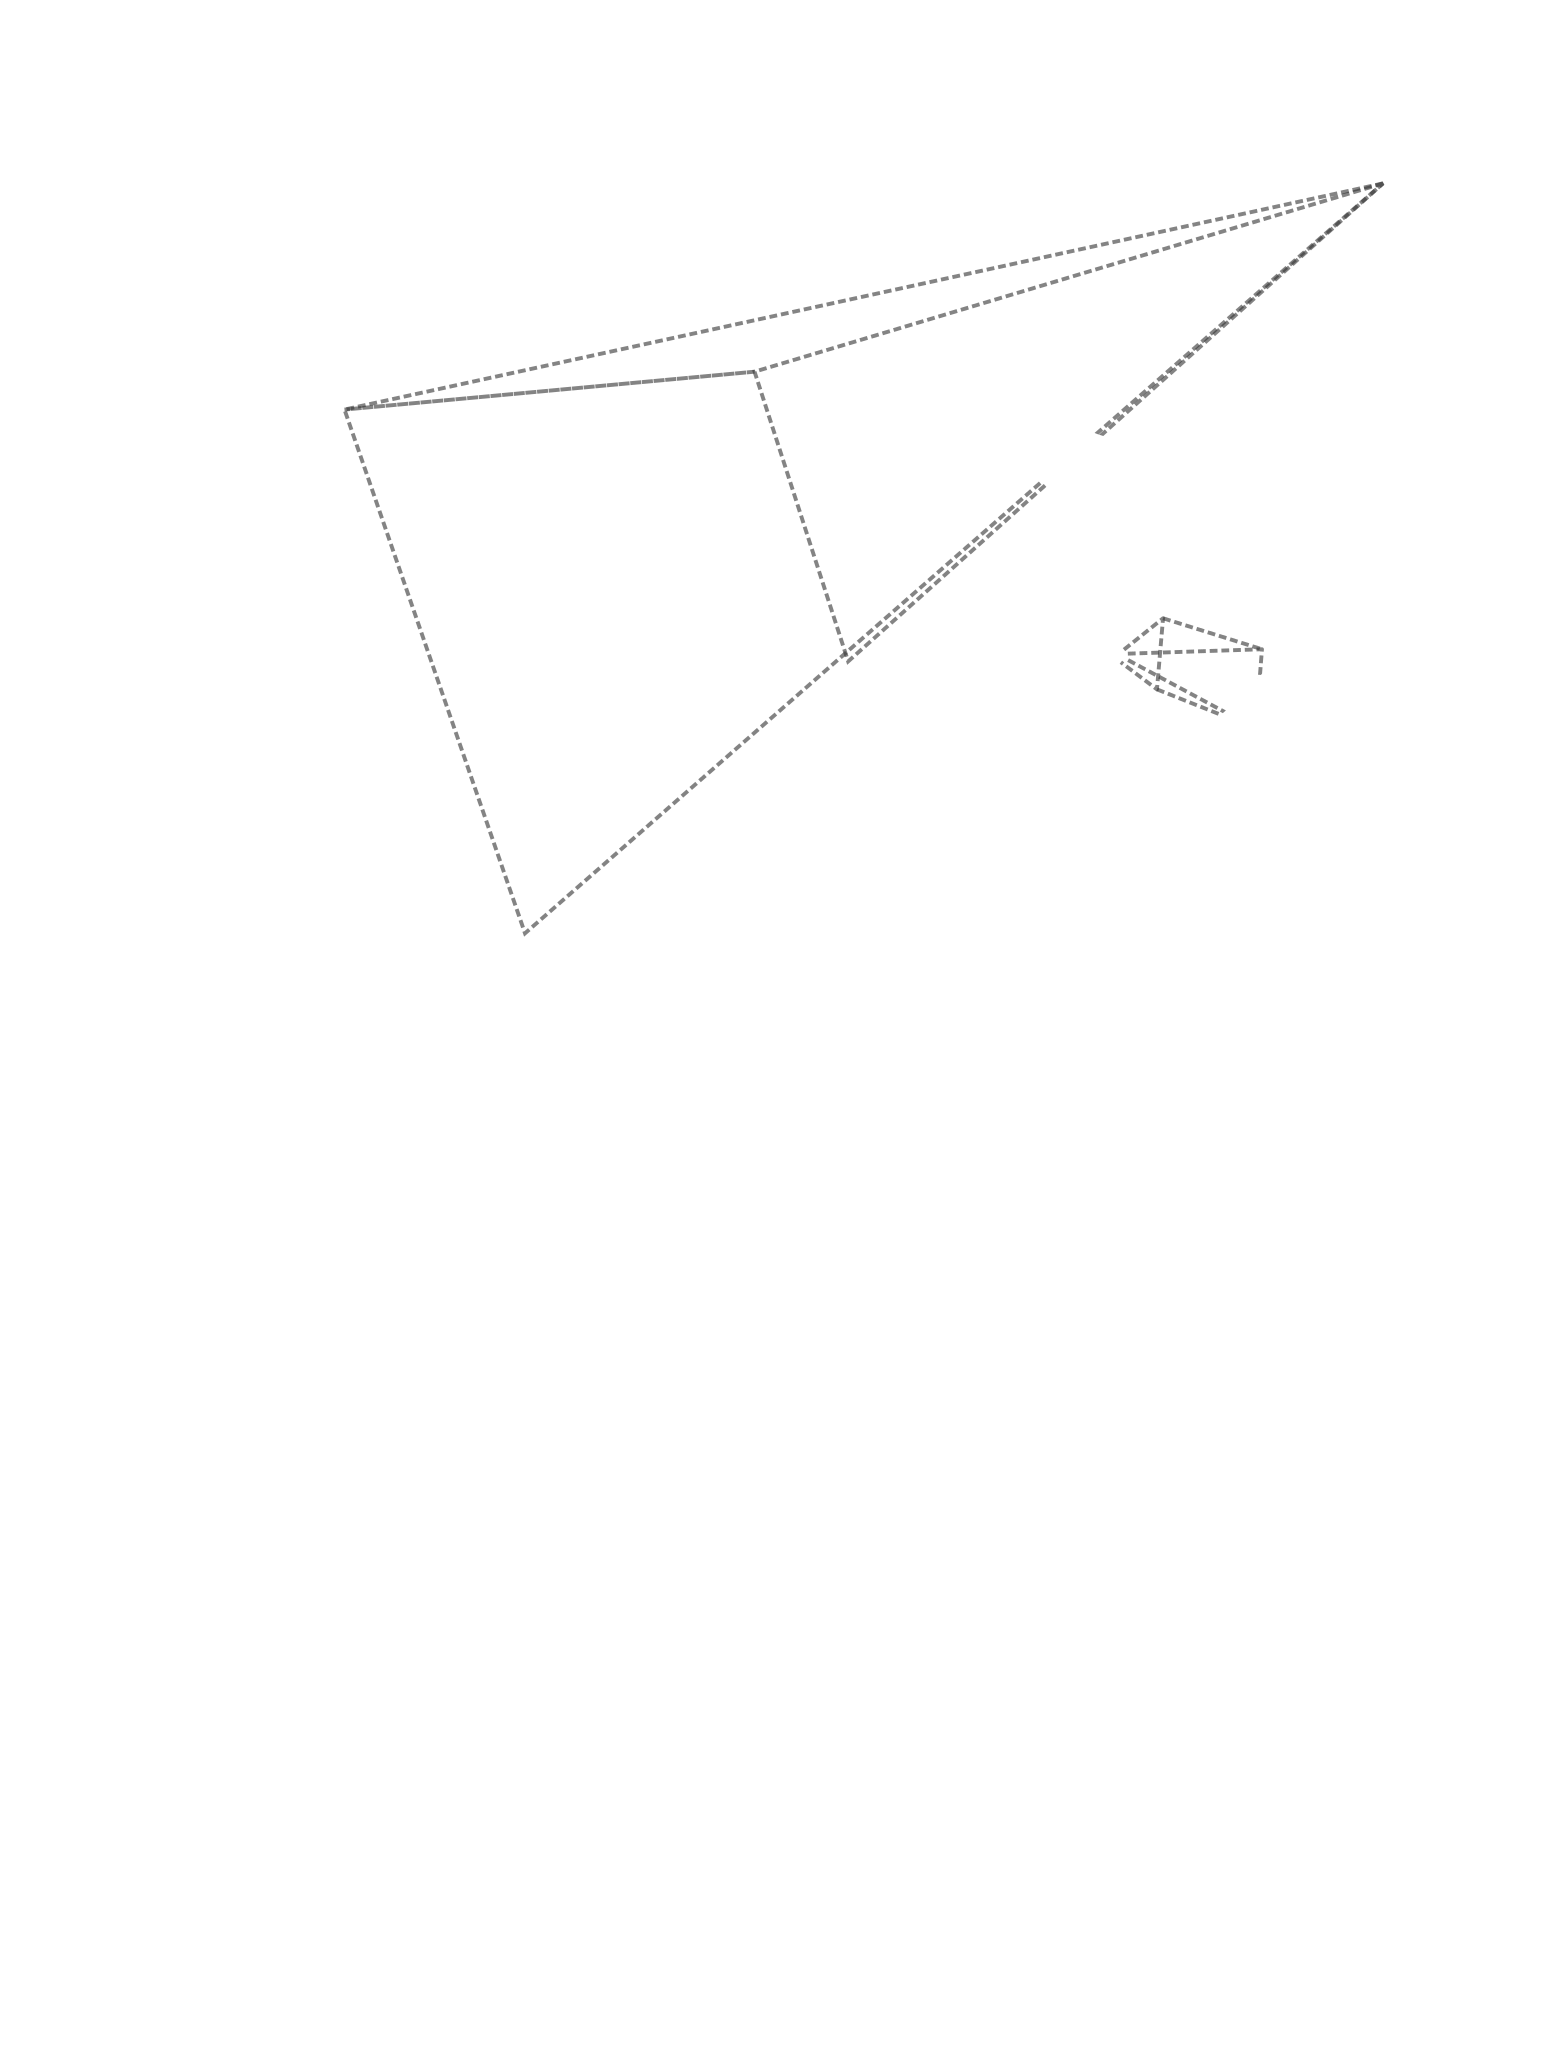
\includegraphics[width=\linewidth]{situation-assessment}

            {\tiny
            \begin{itemize}
                \item real-time situation assessment
                \item geometric reasoning
                \item perspective-taking
            \end{itemize}
            }

        \end{column}
        \begin{column}{0.4\linewidth}

            \begin{figure}

                \resizebox{\columnwidth}{!}{%
                    \begin{tikzpicture}[
                            yscale=1.3,
                            >=latex,
                            every edge/.style={<-, draw, very thick},
                            every node/.style={draw, font=\sf, node distance=0.5, rounded corners,
                            align=center, inner sep=5pt,fill=hriSec2Dark!50},
                            classof/.style={<-, draw=black!60, dashed},
                            property/.style={<-, draw=hriSec2Comp},
                            propname/.style={above, draw=none, fill=none, font=\tt, inner sep=2pt},
                            instance/.style={draw=hriSec1Dark, font=\sf, node distance=0.5, rounded corners,
                            align=center, inner sep=5pt, fill=none}]

                        \node[fill=hriSec2Comp!50] (thing) {\textbf{thing}};
                        \node [fill=hriSec3CompDark!50, node distance=1.8, below left=of
                        thing](sthing) {place} edge[dashed] (thing);
                        \node [fill=hriSec3CompDark!50, below left=of sthing] (agent) {agent} edge (sthing);
                        \node [fill=hriSec3CompDark!50, below=of sthing] (artifact) {artifact} edge (sthing);
                        \node [fill=hriSec3CompDark!50, below right=of sthing] (location) {physical
                        support} edge (sthing);
                        \node [fill=hriSec3CompDark!50, below right=of artifact] (table) {table}
                        edge (location) edge (artifact);


                        \node [node distance=1, below right=of thing] (tthing) {temporal thing} edge (thing);
                        \node [below right=of tthing] (evt) {event} edge[dashed] (tthing);
                        \node [below right=of evt] (act) {action} edge (evt);

                        \uncover<2->{
                            \draw[dotted, thick] (-8,-3.8) -- +(16, 0);

                            \node [instance, below=3 of agent] (human) {human\_1} edge[classof, bend left] (agent);
                            \node [instance, above left=of human] (human2) {human\_2} edge[classof, bend left] (agent);
                            \node [instance, above right=of human, anchor=south] (robot) {myself} edge[classof, bend left] (agent);
                            \node [instance, right=of human, anchor=north west] (book) {book\_game\_thrones}
                            edge[classof] (artifact);
                            \node [instance, right=2 of robot] (ikea) {ikea\_table} edge[classof, bend
                            right] (table);
                            \node [instance, right=2 of book] (brown) {brown} edge[property] node[propname] {hasColor} (book);


                        }
                        \uncover<3->{
                            \draw[dotted, thick] (-8,-6.2) -- +(16, 0);

                            \node [instance, below=5 of act] (moving) {move\_act\_42} edge[classof] (act);
                            \path (moving.west) edge [property, out=180, in=-80, looseness=1] node[propname,below] {currentlyPerforms} (human.230);
                            \path (human.280) edge [property, out=-80, in=-90, looseness=3.5] node[propname,right] {looksAt} (robot.south);
                            \path (ikea.south) edge [property, out=-90, in=-80, looseness=2.5] node[propname, auto] {isOn} (book.320);
                        }
                    \end{tikzpicture}
                    }

            \end{figure}

            {\tiny
            \begin{itemize}
                \item ontologies
                \item real-time symbolic reasoning
                \item theory of mind
            \end{itemize}
            }

        \end{column}
        \begin{column}{0.3\linewidth}
            \begin{figure}
                \resizebox{0.7\columnwidth}{!}{%


                    \begin{tikzpicture}[
                            >=latex,
                            every edge/.style={draw, very thick},
                            skill/.style={draw, rounded corners, align=center, inner sep=5pt, fill=black!20},
                            label/.style={midway, align=center, font=\scriptsize, above},
                            subpart/.style={rounded corners, draw, align=center, font=\scriptsize, fill opacity=0.5, text opacity=1, fill=white!50}]

                        %%% PARSING

                        \node at (0,0)[skill, fill=hriSec3CompDark!50] (prepro) {Pre-processing};
                        \node [left=0.7 of prepro] (input) {\textbf{Input}};
                        \path (input) edge [->] (prepro);

                        %\path (spark.100) edge [->, bend right] node[label] {symbolic \\ facts} (oro);
                        \node [below =0.4 of prepro, skill, fill=hriSec3CompDark!50] (parsing) {Parsing};
                        \path (prepro) edge [->] (parsing);

                        \coordinate (base-onto) at (3,0);

                        %%% RESOLUTION
                        \uncover<2->{
                            \node [below=0.4 of parsing, skill, fill=hriSec3!50, minimum height=4cm, minimum width=5cm] (resolution) {};
                            \node [subpart, below=0.2 of resolution.115] (pron) {Pronouns \& \\ anaphora resolution};
                            \node [subpart, below=0.2 of pron] (noun) {Noun phrase \\ resolution};
                            \node [subpart, right=0.3 of noun, anchor=north west] (discr) {Discrimination};
                            \node [subpart, below=0.2 of noun] (verb) {Verbal phrase \\ resolution};
                            \node [subpart, cylinder, shape border rotate=90, aspect=0.5, below=0.2 of discr] (actions) {Actions};
                            \path (pron) edge [->] (noun);
                            \path (noun) edge [->] (discr);
                            \path (noun) edge [->] (verb);
                            \path (verb) edge [dashed, <->] (actions);
                            \path (pron) edge [dashed, <->] node[label] {queries} (pron -| base-onto);
                            \path (noun.20) edge [dashed, <->] node[label] {queries} (noun.20 -| base-onto);
                            \path (discr) edge [<->] (discr -| base-onto);

                            \node [left=0.2 of resolution.west, rotate=90, anchor=south] {Resolution};
                            \path (parsing) edge [->] (pron);
                        }

                        %%% INTERPRETATION
                        \uncover<3->{
                            \node [skill, below=0.4 of resolution,minimum width=5cm, minimum height=3cm] (interp) {};
                            \node [subpart, below=0.2 of interp.north] (content) {Content analysis};
                            \node [below=0.6 of content.south west, subpart] (question) {Question \\ handler};
                            \node [below=0.6 of content.south east, subpart] (stat) {Statement \\ builder};
                            \path (content) edge [->] node[label, left] {question} (question);
                            \path (content) edge [->] node [label, right] {goal | statement} (stat);
                            \path (stat) edge [->] node [label] {asserts} (stat -| base-onto);

                            \node [left=0.2 of interp.west, rotate=90, anchor=south] {Interpretation};

                            \path (verb) edge [->] (content);
                            \path (question) edge [dashed, bend right, <->] node[label] {queries} (question.south -| base-onto);
                        }

                        %%% ONTOLOGY
%                        \uncover<2->{
%                            \node at (resolution.north -| base-onto) [rotate=-90, skill, minimum height=2cm, minimum width=7cm, fill=hriSec3!50, anchor=south west] (onto) {Ontology server};

%                        }

                        %%% VERBALIZATION
                        \uncover<4->{
                            \node [below=0.7 of interp, skill, fill=hriSec2Dark!50] (verb) {Verbalization};
                            \path (question) edge [->] (verb);
                            \path (stat) edge [->] (verb);
                            \path (discr.south east) edge [black!50, dashed, bend left, <->] (verb.north east);
                            \node [right=0.7 of verb] (output) {\textbf{Output}};
                            \path (verb) edge [->] (output);
                        }
                    \end{tikzpicture}
                    }
                \end{figure}

            {\tiny
            \begin{itemize}
                \item symbolic grounding
                \item natural language processing
                \item interactive disambiguation and concept learning
            \end{itemize}
            }


            \end{column}
        \end{columns}



        %\badge{europe_phd}
    \end{frame}

\begin{frame}{Symbolic social cognition}

Main contributions:

    \begin{enumerate}
        \item \textbf{ontologies} to model the robot knowledge
        \item \textbf{situation assessment} using real-time 3D models of the
            environment to generate symbolic facts
        \item \textbf{perspective taking} and \textbf{theory of mind}: generate and
            maintain symbolic knowledge models for all the agents
        \item Application: \textbf{perspective-aware situated dialogue} with real-time \textbf{symbolic
            grounding}
    \end{enumerate}

Impact:
    \begin{itemize}
        \item Prix GdR Meilleure thèse
        \item 10+ publications, incl. \emph{Intl. Journal of Social Robotics};
            \emph{IROS}x2; \emph{HRI}; \emph{RoMAN}x2; \textbf{500+ citations}
    \end{itemize}
\end{frame}

%%%%%%%%%%%%%%%%%%%%%%%%%%%%%%%%%%%%%%%%%%%%%%%%%%%%%%%%%%%%%%%%%%%%%%%%%%
\section{2. Real-world social autonomy}

\begin{frame}<6>{Architecture for social \& autonomous interaction}

    \begin{center}

     \begin{columns}
         \begin{column}{0.5\linewidth}

        \resizebox{\columnwidth}{!}{%

            
            \alt<7>{\newcommand{\dimming}{10}}{\newcommand{\dimming}{50}}

            \tikzset{subpart/.style={draw, font=\scriptsize, fill opacity=0.5, text opacity=1, fill=white!50}}

            \begin{tikzpicture}[
                    >=latex,
                    every edge/.style={draw, very thick},
                    skill/.style={draw, rounded corners, align=center, inner sep=5pt, fill=black!20},
                label/.style={midway, align=center, font=\scriptsize, fill=white}]

                %%% Separation between deliberative layer and sensori-motor layer
                \draw[dotted, thick] (-8,-5) -- (12, -5);

                %%% SPARK
                \uncover<2->{
                    \node at (4,-3.5)[skill, fill=hriSec3!\dimming] (spark) {%
                    \begin{tikzpicture}
                        \node at (0,0) (geom) {Geometric \& Temporal Reasoning -- {\tt spark}};
                        \node [subpart, below=0.2 of geom.south west, anchor=north west] (world-update) {Sensors fusion};
                        \node [subpart, right=0.2 of world-update] (geom-model) {Geometric model of the environment};
                        \node [subpart, right=0.2 of geom-model] (fact-prod) {Symbolic facts production};
                    \end{tikzpicture}
                };
                }

                %%% LOWLEVEL
                \node [skill, below=0.7 of spark,fill=gray!\dimming] (lowlevel) {%
                    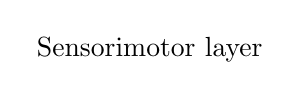
\begin{tikzpicture}
                        \node at (0,0) (sensori) {Sensorimotor layer};
                        %\node [subpart, below=0.2 of sensori.south west, anchor=north west, align=left] (perception) {{\bf Perception} \\ 2D markers, RGB-D, motion capture};
                        %\node [subpart, align=right, right=0.2 of perception] {{\bf Actuation} \\ Head's pan-tilt unit, grippers, arms, wheels};
                    \end{tikzpicture}
                };

                \uncover<2->{
                \path (lowlevel) edge [->] (spark);
                }

                %%% ORO
                \uncover<3->{
                \node at (0,0)[skill, ultra thick, fill=hriSec2Dark!50] (oro)
                {Symbolic facts \\ and beliefs management -- {\tt oro}};
                \path (spark.100) edge [->, bend right] node[label] {symbolic \\ facts} (oro);
                }

                %%% HATP
                \uncover<5->{
                \node at (-6, 2.5)[skill, fill=hriSec1!\dimming] (hatp) {Human-aware
                symbolic \\task planning -- {\tt hatp}};
                \path (hatp) edge [<->, bend right] node[label] {world model and \\ agents beliefs} (oro.170);
                }

                %%% DIALOGS
                \uncover<4->{
                \node at (-6, -3) [skill, fill=hriSec3Dark!50] (dialogs)
                {Dialogue processing\\{\tt dialogs}};
                \path (dialogs) edge [<->, bend left] node[label] {natural language \\ grounding} (oro.190);
                }
                %%% SHARY
                \uncover<5->{
                \node at (4,4.5)[skill, fill=hriSec1Comp!\dimming] (shary) {%
                    \begin{tikzpicture}
                        \node at (0,0) (exec) {Execution Controller -- {\tt shary} | {\tt pyrobots}};
                        \node [subpart, below=0.2 of exec.south west, anchor=north west] (plans) {Goal \& Plans \\ management};
                        \node [subpart, right=0.2 of plans] (sit-asses) {Situation assessment \\ and context management};
                        \node [subpart, right=0.2 of sit-asses] {Action instantiation, \\ execution and monitoring};
                    \end{tikzpicture}
                };
                \path (shary) edge [<->, bend left] node[label] {events, \\ world model and \\ agents beliefs} (oro);
                \path (shary) edge [<->, bend left, looseness=0.8] node[label] {action monitoring \\ and management of \\ position hypotheses} (spark);
                \path (shary.west) edge [<->, bend right] node[label] {shared \\ plans} (hatp);
                }
                %%% MHP
                \uncover<6->{
                \node at (9,0)[skill, fill=hriSec3CompDark!\dimming] (mhp) {Human-aware Motion \\ and Manipulation Planning\\{\tt mhp}};
                \path (shary.340) edge [<->, bend left] node[label] {motion plan \\ requests} (mhp);
                \path (spark.5) edge [->, bend right] node[label] {environment\\model} (mhp);
                \path (lowlevel.east) edge [<-, bend right=60, looseness=1.3] node[label] {atomic\\actions} (mhp.south east);
                }



            \end{tikzpicture}
        }
         \end{column}
         \begin{column}{0.5\linewidth}
             \centering
             \resizebox{\columnwidth}{!}{%
                 \begin{tikzpicture}[
                         >=latex,
                     every edge/.style={draw, ultra thick, ->},
                     every node/.style={align=center},
                     robot/.style={fill=hriSec2Comp!50},
                     plan/.style={draw,
                      thick,  
                      circle, 
                      font=\sf,
                      align=center,
                      fill=hriSec3CompDark!50, 
                      minimum size=1cm, 
                      inner sep=0.1cm}
                  ]

                     \coordinate (figbottom) at (-0.5, -28.5);


                     \fill[gray!10!white] (4.6,.5) rectangle (figbottom);

                     \path (-0.5,0) edge (figbottom) node[sloped, above left, rotate=90] {\large\bf time};

                     \node at (2,0) (percept) {\bf Perception};
                     \node[below=0.5 of percept.south west, anchor=mid] {camera};
                     \node[below=0.5 of percept.south east, anchor=mid] {3D model};

                     \node[right=4 of percept, minimum width=2.5cm] (kb) {\bf Knowledge};
                     \node[below=0.5 of kb.south west, anchor=mid east] (kbr) {robot};
                     \node[below=0.5 of kb.south east, anchor=mid west] (kbh) {human};
                     \draw[dotted] (kbr) to (figbottom -| kbr);
                     \draw[dotted] (kbh) to (figbottom -| kbh);

                     \fill[gray!10!white] (12,.5) rectangle (17,0 |- figbottom);
                     \node[right=4.5 of kb] (plan) {\bf Plan};
                     \node[below=0.5 of plan.south west, anchor=mid east] (probot) {robot};
                     \node[below=0.5 of plan.south east, anchor=mid west] (phuman) {human};
                     \draw[dotted] (probot) to (figbottom -| probot);
                     \draw[dotted] (phuman) to (figbottom -| phuman);

                     \node[right=5 of plan] (action) {\bf Actions};
                     \node[below=0.5 of action.south west, anchor=mid east] (arobot) {robot};
                     \node[below=0.5 of action.south east, anchor=west] (ahuman) {human\\(monitoring)};
                     \draw[dotted] (arobot) to (figbottom -| arobot);
                     \draw[dotted] (ahuman) to (figbottom -| ahuman);

                     \draw[dashed] (-0.6,-1.2) --(24, -1.2);

                     \node[anchor=east] at (-0.5, -3) (t1) {\Large $t_1$};
                     \node[anchor=east, below=6 of t1] (t2) {\Large $t_2$};
                     \node[anchor=east, below=6 of t2] (t3) {\Large $t_3$};
                     \node[anchor=east, below=4 of t3] (t4) {\Large $t_4$};
                     \node[anchor=east, below=5 of t4] (t5) {\Large $t_5$};

                     %%%%%%%%%%%%%%%%%%%%%%%%%%%%%%%%%%%%%%%%%%%%%%%%%%%%%%%%%%%%%%%%%%%%%%%%%%%%%%%%%%%%%%%%%%%%
                     %%% PERCEPTIONS
                     %%%%%%%%%%%%%%%%%%%%%%%%%%%%%%%%%%%%%%%%%%%%%%%%%%%%%%%%%%%%%%%%%%%%%%%%%%%%%%%%%%%%%%%%%%%%

         \node at (t1 -| percept) (cam1) {\includegraphics[height=2cm]{cleantable/manip_run_cam1.png}};
         \node at (t2 -| percept) (cam2) {\includegraphics[height=2cm]{cleantable/manip_run_cam2.png}};
         \node at (t3 -| percept) (cam3) {\includegraphics[height=2cm]{cleantable/manip_run_cam3.png}};
         \node at (t4 -| percept) (cam4) {\includegraphics[height=2cm]{cleantable/manip_run_cam4.png}};
         \node at (t5 -| percept) (cam5) {\includegraphics[height=2cm]{cleantable/manip_run_cam5.png}};

         %%%%%%%%%%%%%%%%%%%%%%%%%%%%%%%%%%%%%%%%%%%%%%%%%%%%%%%%%%%%%%%%%%%%%%%%%%%%%%%%%%%%%%%%%%%%
         %%% KNOWLEDGE
         %%%%%%%%%%%%%%%%%%%%%%%%%%%%%%%%%%%%%%%%%%%%%%%%%%%%%%%%%%%%%%%%%%%%%%%%%%%%%%%%%%%%%%%%%%%%

         \node[fill=white,align=left] at (cam1 -| kbr) (kb1) {\stmt{TAPE isVisible true}\\
                                                    \stmt{TAPE isReachable true}\\
                                                    \stmt{TAPE isOn TABLE}\\
                                                    \stmt{BIN isVisible true}\\
                                                    \stmt{BIN isReachable false}};

         \node[fill=white,align=left] at (cam1 -| kbh) {\stmt{TAPE isVisible true}\\
                                                    \stmt{TAPE isReachable false}\\
                                                    \stmt{TAPE isOn TABLE}\\
                                                    \stmt{BIN isVisible true}\\
                                                    \stmt{BIN isReachable true}};

         \node[fill=white,align=left] at (cam2 -| kbr) (kb2) {\stmt{ROBOT hasInHand TAPE}};


         \node[fill=white,align=left] at (cam3 -| kbr) {\stmt{TAPE isReachable true}\\
                                        \stmt{TAPE isVisible true} \\
                                        \stmt{TAPE isOn TABLE}};

         \node[fill=white,align=left ] at (cam3 -| kbh) (kb3) {\stmt{TAPE isReachable true}\\
                                         \stmt{TAPE isVisible true}};

         \node[fill=white,align=left] at (cam4 -| kbh) (kb4) {\stmt{HUMAN hasInHand TAPE}};

         \node[fill=white,align=left] at (cam5 -| kbr)  {\stmt{TAPE isIn BIN}};
         \node[fill=white,align=left] at (cam5 -| kbh) (kb5) {\stmt{TAPE isIn BIN}};

         %%%%%%%%%%%%%%%% %%%%%%%%%%%%%%%%%%%%%%%%%%%%%%%%%%%%%%%%%%%%%%%%%%%%%%%%%%%%%%%%%%%%%%%%%%%%
         %%% PLANS
         %%%%%%%%%%%%%%%%%%%%%%%%%%%%%%%%%%%%%%%%%%%%%%%%%%%%%%%%%%%%%%%%%%%%%%%%%%%%%%%%%%%%%%%%%%%%

         \node[fill=gray!10!white,below=1 of plan] (incoming) {\bf \Large Incoming goal \\ \it Clean the table!};

         \node[anchor=north, plan, robot] at (cam1.south -| probot) (pr1) {\bf TAKE\\TAPE\\TABLE};
         \node[anchor=north, plan, robot] at (cam2.south -| probot)  (pr2) {\bf PUTRV\\TAPE\\TABLE} edge[<-] (pr1);
         \node[anchor=north, plan] at (cam3.south -| phuman) (ph1) {\bf TAKE\\TAPE\\TABLE} edge[<-] (pr2);
         \node[anchor=north, plan]  at (cam4.south -| phuman) (ph2) {\bf PUT\\TAPE\\BIN} edge[<-] (ph1);

         \node[fill=gray!10!white,anchor=north] at (cam5.south -| plan) (done) {\bf \Large Goal completed};

         %%%%%%%%%%%%%%%%%%%%%%%%%%%%%%%%%%%%%%%%%%%%%%%%%%%%%%%%%%%%%%%%%%%%%%%%%%%%%%%%%%%%%%%%%%%%
         %%% ACTIONS
         %%%%%%%%%%%%%%%%%%%%%%%%%%%%%%%%%%%%%%%%%%%%%%%%%%%%%%%%%%%%%%%%%%%%%%%%%%%%%%%%%%%%%%%%%%%%

         \only{
             \node[fill=white] at (pr1 -| arobot) (ep1) {\it evaluate pre-conditions};

         \node[below=0.1 of ep1] (mhp1) {%
             \begin{tikzpicture}
                 \node[fill=white] (title) {\bf motion planning};
                 \node[below=0.1 of title.south west, label=below:{\tt PICK\_GOTO}] (mapg) {\includegraphics{cleantable/MHP_ARM_PICK_GOTO}};
                 \node[fill=white,right=of mapg, label=below:{\tt TAKE\_TO\_FREE}] (mattf) {\includegraphics{cleantable/MHP_ARM_TAKE_TO_FREE}} edge[<-] (mapg);
             \end{tikzpicture}
         };
         \node[fill=white,below=0.1 of mhp1] (me1) {\bf motion execution};
         \node[fill=white,below=0.1 of me1] (ae1) {\it assess post-conditions};
     }
     %%%%%%%%%%%%%%%%%%%%%%%%%%%%%%%%%%%%%%%%%%%%%%%%%%%%%%%%%%%%%%%%%%%%%%%%%%%%%%%%%%%%%%%%%%%%%
         \only{
             \node[fill=white] at (pr2 -| arobot) (ep2) {\it evaluate pre-conditions};

         \node[below=0.1 of ep2] (mhp2) {%
             \begin{tikzpicture}
                 \node[fill=white] (title) {\bf motion planning};
                 \node[fill=white,below=0.1 of title, label=below:{\tt ESCAPE}] (maeo) {\includegraphics{cleantable/MHP_ARM_ESCAPE_OBJECT}};
                 \node[left=of maeo, label=below:{\tt PLACE\_FROM\_FREE}] (mapff) {\includegraphics{cleantable/MHP_ARM_PLACE_FROM_FREE}} edge (maeo);
                 \node[fill=white,right=of maeo, label=below:{\tt TO\_FREE}] (maf) {\includegraphics{cleantable/MHP_ARM_FREE}} edge[<-] (maeo);
             \end{tikzpicture}
         };
         \node[fill=white,below=0.1 of mhp2] (me2) {\bf motion execution};
         \node[fill=white,below=0.1 of me2] (ae2) {\it assess post-conditions};
     }
     %%%%%%%%%%%%%%%%%%%%%%%%%%%%%%%%%%%%%%%%%%%%%%%%%%%%%%%%%%%%%%%%%%%%%%%%%%%%%%%%%%%%%%%%%%%%%

         \node[anchor=north] at (ph1 -| ahuman) (wait1) {%
             \begin{tikzpicture}
                 \node[fill=white] (title) {\it wait for pick\\ {\tt TAPE} \it from {\tt TABLE}};
                 \node[below=0.1 of title] {\includegraphics{cleantable/wait_for_pick}};
             \end{tikzpicture}
         };

         \node[anchor=north] at (ph2 -| ahuman) (wait2) {%
             \begin{tikzpicture}
                 \node[fill=white] (title) {\it wait for put\\ {\tt TAPE} \it into {\tt BIN}};
                 \node[below=0.1 of title] {\includegraphics{cleantable/wait_for_throw}};
             \end{tikzpicture}
         };


         %%%%%%%%%%%%%%%%%%%%%%%%%%%%%%%%%%%%%%%%%%%%%%%%%%%%%%%%%%%%%%%%%%%%%%%%%%%%%%%%%%%%%%%%%%%%
         %%% FLOW
         %%%%%%%%%%%%%%%%%%%%%%%%%%%%%%%%%%%%%%%%%%%%%%%%%%%%%%%%%%%%%%%%%%%%%%%%%%%%%%%%%%%%%%%%%%%%
         \draw[dotted, ->, in=45, out=180] (incoming.west) to (kb1);
         \draw[dotted, ->, bend right] (kb1) to (pr1);
         \draw[dotted, ->, bend left] (pr1) to (ep1);
         \draw[dotted, ->, in=45, out=180] (ae1.west) to (kb2);
         \draw[dotted, ->, bend right] (kb2) to (pr2);
         \draw[dotted, ->, bend left] (pr2) to (ep2);
         \draw[dotted, ->, in=45, out=180] (ae2.west) to (kb3);
         \draw[dotted, ->, bend right] (kb3) to (ph1);
         \draw[dotted, ->, bend left] (ph1) to (wait1);
         \draw[dotted, ->, in=-20, out=180] (wait1.west) to (kb4.east);
         \draw[dotted, ->, bend right] (kb4) to (ph2);
         \draw[dotted, ->, bend left] (ph2) to (wait2);
         \draw[dotted, ->, in=20, out=180] (wait2.west) to (kb5);
         \draw[dotted, ->, bend left] (kb5.east) to (done.north);


     \end{tikzpicture}
      }
         \end{column}
     \end{columns}
    \end{center}

\end{frame}

\begin{frame}{Expert-in-the-loop machine learning}

    \begin{columns}
        \begin{column}{0.5\linewidth}
                \centering
                \includegraphics[height=3cm]{couch25k/hri.jpg}
        \end{column}
        \begin{column}{0.5\linewidth}
                \centering
                \includegraphics[height=3cm]{couch25k/supervised.jpg}
        \end{column}
    \end{columns}
        \centering
        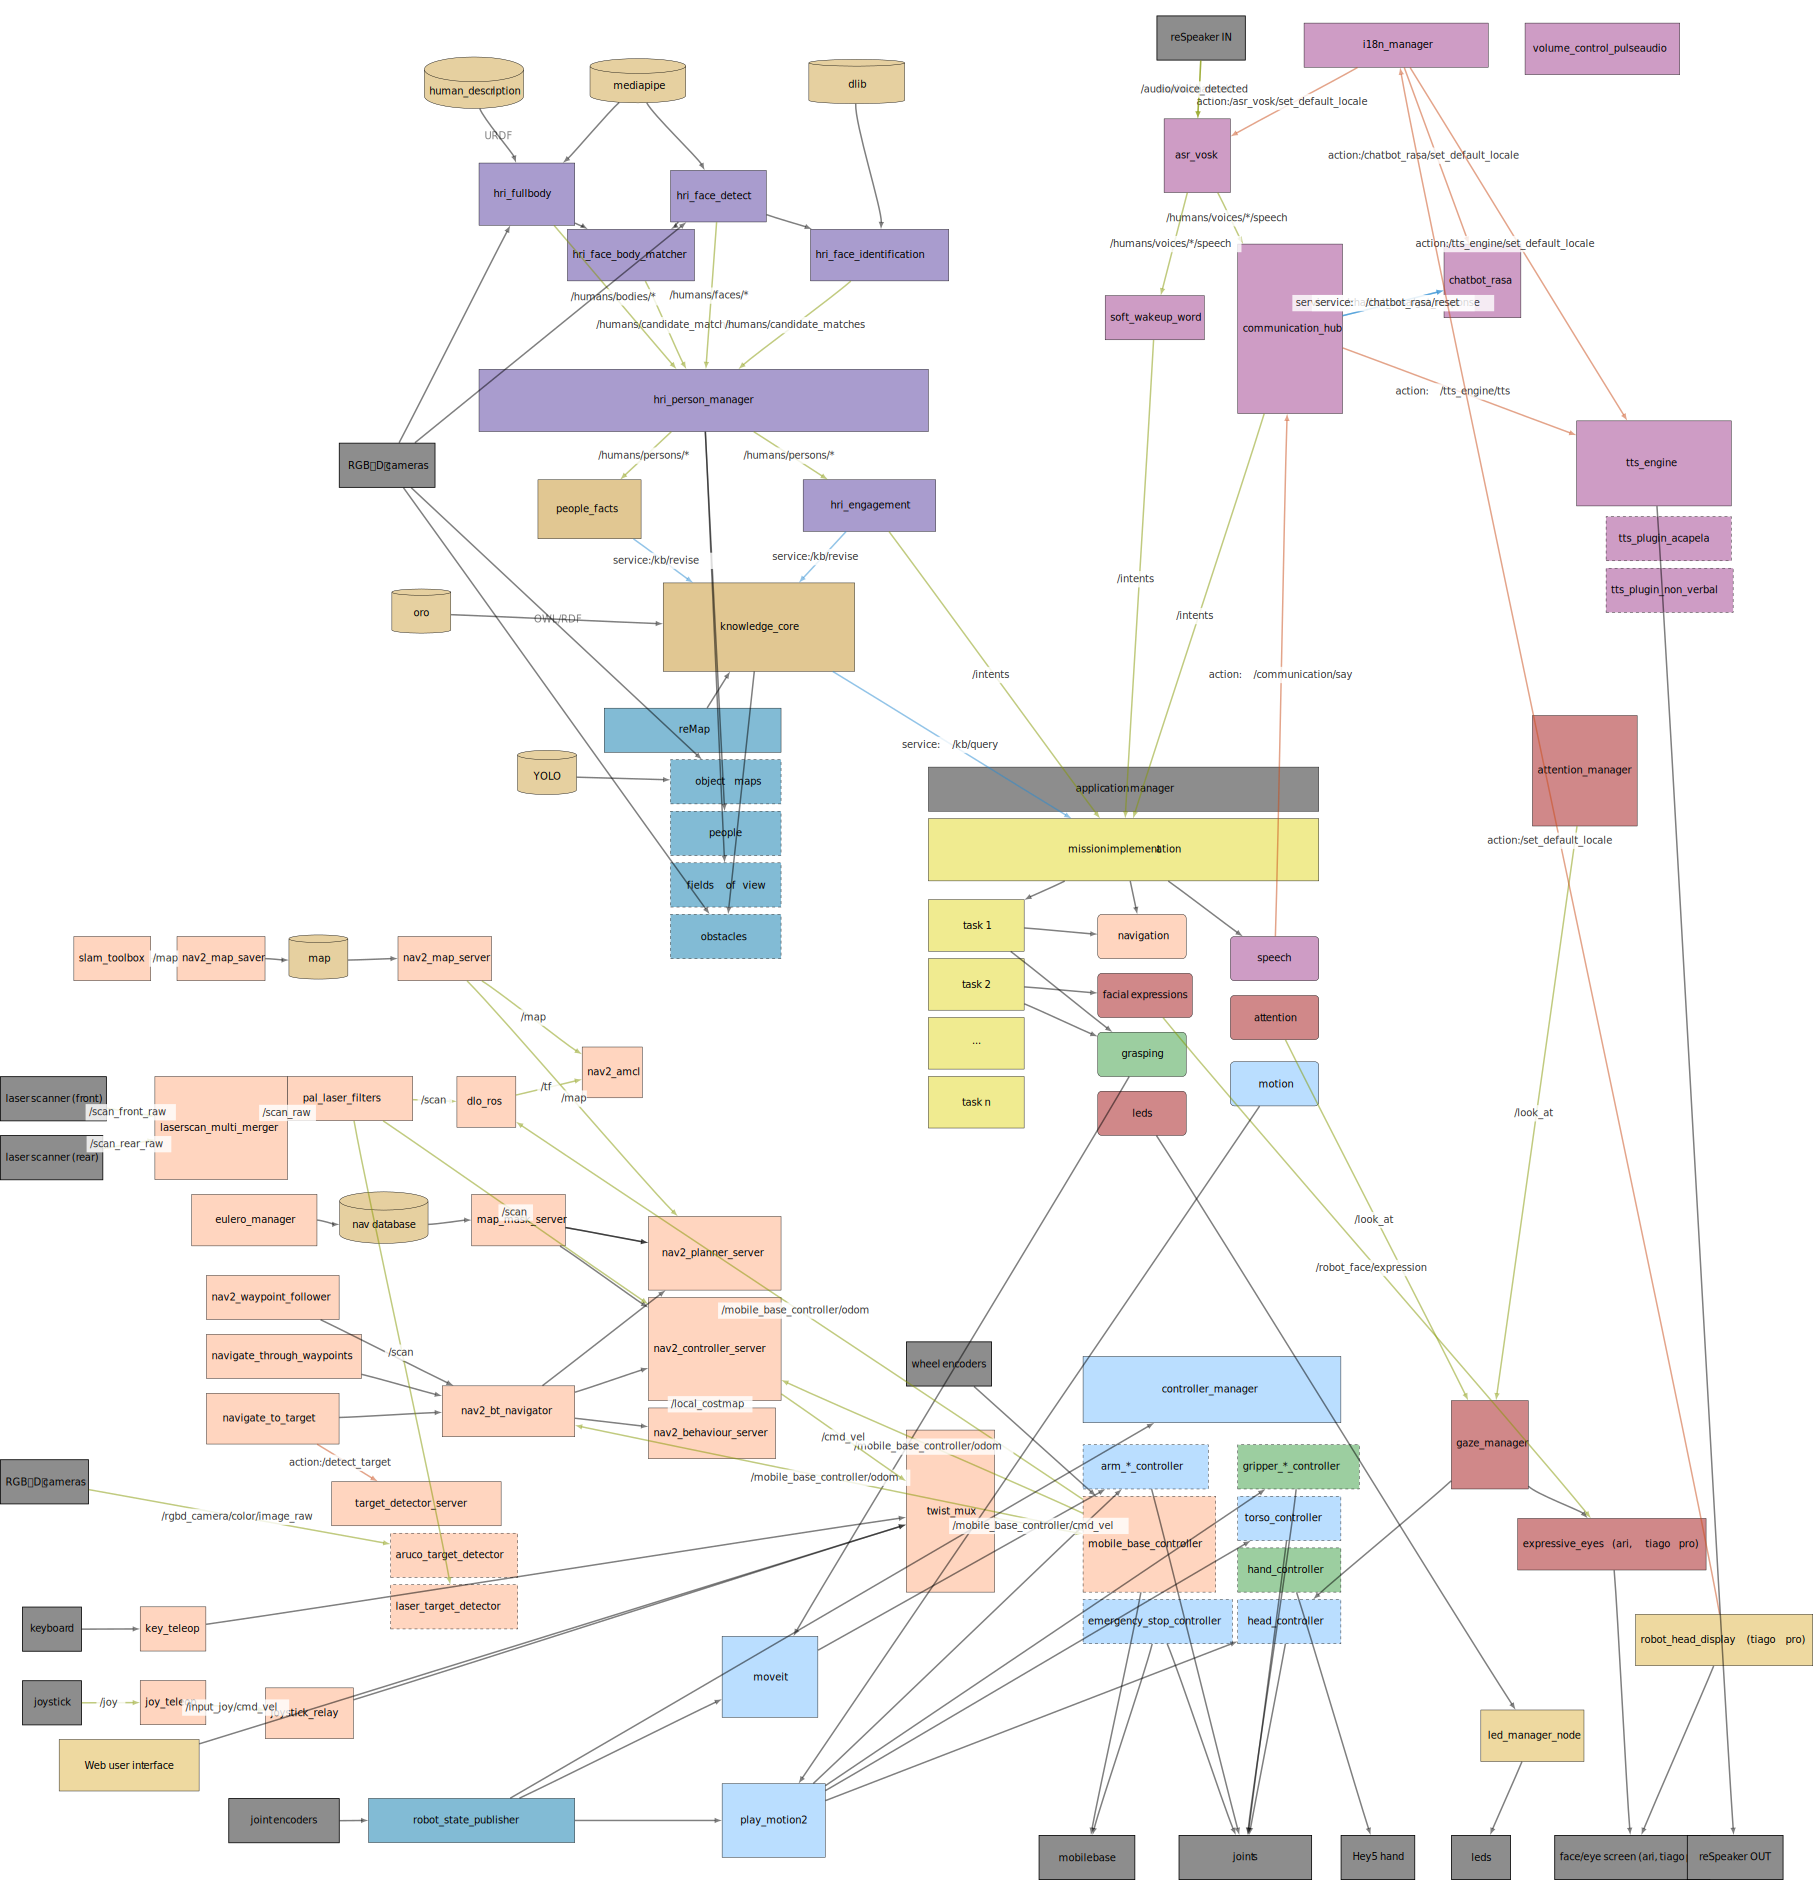
\includegraphics[height=4cm]{couch25k/architecture.pdf}
\end{frame}

\begin{frame}{Real-world social autonomy}

Main contributions:

    \begin{enumerate}
        \item \textbf{ontologies} to model the robot knowledge
        \item \textbf{situation assessment} using real-time 3D models of the
            environment to generate symbolic facts
        \item \textbf{perspective taking} and \textbf{theory of mind}: generate and
            maintain symbolic knowledge models for all the agents
        \item Application: \textbf{perspective-aware situated dialogue} with real-time \textbf{symbolic
            grounding}
    \end{enumerate}

Impact:
    \begin{itemize}
        \item Prix GdR Meilleure thèse
        \item 10+ publications, incl. \emph{Intl. Journal of Social Robotics};
            \emph{IROS}x2; \emph{HRI}; \emph{RoMAN}x2; \textbf{500+ citations}
    \end{itemize}
\end{frame}


\section[cHRI]{...to child-robot interaction...}

\imageframe[color=black]{experiments-cHRI}

\section[Data-driven HRI]{...to data-driven HRI: interactive reinforcement learning}
{
    \paper{Winkle et al. \textbf{In-Situ Learning from a Domain Expert for Real World Socially Assistive Robot Deployment}
    RSS 2020}
    \fullbackground[scale=0.9]{couch25k/finalactiondist.png}
\begin{frame}{}
\end{frame}
}
{
    \paper{Winkle et al. \textbf{In-Situ Learning from a Domain Expert for Real World Socially Assistive Robot Deployment}
    RSS 2020}
    \fullbackground[scale=0.9]{couch25k/fullcomp_lbmr.png}
\begin{frame}{}
\end{frame}
}

\section[Social dynamics]{Data-driven HRI: social dynamics}
{
    \paper{Lemaignan et al. \textbf{The PInSoRo dataset [...]} PLOS ONE
    2018}
    \fullbackground[scale=0.9]{pinsoro/annotator.jpg}
\begin{frame}{}
\end{frame}
}

%\videoframe[0.56]{figs/kinematics_social_dynamics/clip_skel_01.mp4}

%%%%%%%%%%%%%%%%%%%%%%%%%%%%%%%%%%%%%%%%%%%%%%%%%%%%%%%%

%\videoframe[0.56]{figs/kinematics_social_dynamics/clip_01.mp4}

%%%%%%%%%%%%%%%%%%%%%%%%%%%%%%%%%%%%%%%%%%%%%%%%%%%%%%%%

\videoframe[0.56]{figs/kinematics_social_dynamics/clip_skel_05.mp4}

%%%%%%%%%%%%%%%%%%%%%%%%%%%%%%%%%%%%%%%%%%%%%%%%%%%%%%%%

\videoframe[0.56]{figs/kinematics_social_dynamics/clip_05.mp4}

\imageframe[caption={200 participants, 4 clips each, on MTurk}]{kinematics_social_dynamics/questionnaire.png}
%\imageframe{kinematics_social_dynamics/dataset.png}
%\imageframe[caption={For each construct, calculate $\Delta$ and $\Sigma$}]{kinematics_social_dynamics/dataset-sumdiff.png}

{
    \paper{Bartlett et al. \textbf{What Can You See? Identifying Cues on
Internal States from the Kinematics [...]} Frontiers
2019}
\begin{frame}{EFA: Exploratory Factor Analysis}

\tiny
\rowcolors{2}{gray!25}{white}
\begin{tabular}{lrr|rr|rr}

    {} & \multicolumn{2}{l}{\bf Factor 1\onslide<2->{: imbalance}} &
    \multicolumn{2}{l}{\bf Factor 2\onslide<2->{: (negative) valence}} & \multicolumn{2}{l}{\bf
    Factor 3\onslide<2->{: engagement}} \\
    {} & \emph{full-scene} &  \onslide<3->{\emph{mov.-alone}} & \emph{full-scene} &
    \onslide<3->{\emph{mov.-alone}} & \emph{full-scene} &
    \onslide<3->{\emph{mov.-alone}} \\
\midrule
    \textbf{$\Delta$ Sad       } &      0.41 &  \only<3->{0.52} &           &                  &           &       \\
    \textbf{$\Sigma$ Sad       } &           &                  &      0.72 & \only<3->{ 0.53} &           & \only<3->{ 0.49} \\
    \textbf{$\Delta$ Happy     } &      0.49 &  \only<3->{0.53} &           &                  &           & \\
    \textbf{$\Sigma$ Happy      } &           &                 &           & \only<3->{-0.51} &     -0.55 & \\
    \textbf{$\Delta$ Angry     } &      0.40 &  \only<3->{0.62} &           &                  &           & \\
    \textbf{$\Sigma$ Angry      } &           &                 &      0.81 & \only<3->{ 0.85} &           & \\
    \textbf{$\Delta$ Excited   } &      0.53 &  \only<3->{0.63} &           &                  &           & \\
    \textbf{$\Sigma$ Excited    } &           &                 &           &                  &     -0.71 & \\
    \textbf{$\Delta$ Calm      } &      0.45 &  \only<3->{0.63} &           &                  &           & \\
    \textbf{$\Sigma$ Calm       } &           &  \only<3-> {  } &           & \only<3->{-0.45} &           & \\
    \textbf{$\Delta$ Friendly  } &      0.69 &  \only<3->{0.56} &           &                  &           & \\
    \textbf{$\Sigma$ Friendly   } &           &  \only<3->{   } &           & \only<3->{-0.60} &     -0.43 & \\
    \textbf{$\Delta$ Aggressive} &      0.78 &  \only<3->{0.79} &           &                  &           & \\
    \textbf{$\Sigma$ Aggressive } &           &  \only<3->{   } &      0.80 & \only<3->{ 0.72} &     -0.36 & \\
    \textbf{$\Delta$ Engaged   } &           &  \only<3->{0.39} &           &                  &      0.65 & \only<3->{ 0.52} \\
    \textbf{$\Sigma$ Engaged    } &           &  \only<3->{   } &           &                  &     -0.64 & \only<3->{-0.64} \\
    \textbf{$\Delta$ Distracted} &           &  \only<3->{    } &           &                  &      0.65 & \only<3->{ 0.63} \\
    \textbf{$\Sigma$ Distracted } &           &  \only<3->{   } &      0.63 &                  &           & \only<3->{ 0.82} \\
    \textbf{$\Delta$ Bored     } &           &  \only<3->{0.44} &           &                  &      0.61 & \only<3->{ 0.54} \\
    \textbf{$\Sigma$ Bored      } &           &  \only<3->{   } &      0.58 &                  &      0.48 & \only<3->{ 0.83} \\
    \textbf{$\Delta$ Frustrated} &      0.53 &  \only<3->{0.61} &           &                  &           &       \\
    \textbf{$\Sigma$ Frustrated } &           &  \only<3->{   } &      0.70 & \only<3->{ 0.69} &           &       \\
    \textbf{$\Delta$ Dominant  } &      0.75 &  \only<3->{0.81} &           &                  &           &       \\
    \textbf{$\Sigma$ Dominant   } &           &  \only<3->{   } &      0.53 & \only<3->{ 0.52} &           &       \\
    \textbf{$\Delta$ Submissive} &      0.68 &  \only<3->{0.72} &           &                  &           &       \\
    \textbf{$\Sigma$ Submissive } &          &                  &      0.54 &                  &           &       \\

\end{tabular}

    \note{Very strong correlation: Factor 1: r = 0.94, p < 0.001; for Factor 2: r = 0.84, p < 0.001; for Factor 3: r = 0.81, p < 0.001}

\end{frame}
}

\begin{frame}{Three constructs to rule them all}
        \centering
        \includegraphics[width=0.9\linewidth]{kinematics_social_dynamics/clips.jpg}

    \textbf{Interaction imbalance}
    
    \textbf{Interaction valence}
    
    \textbf{Engagement}

\end{frame}

%\begin{frame}{Mean EFA projection of clips per social situation}
%
%    \only<1>{
%        The 20 clips were labelled after their salient social features
%        (\emph{aggressive}, \emph{excited}, \emph{aimless}, \emph{fun},
%        \emph{cooperative}, \emph{bored}, \emph{dominant}).
%
%        \vspace{2cm}
%        What happen if we project the ratings for 'aggressive' clips,
%        'excited' clips, etc. onto the 3 EFA factors?
%
%    }
%
%    \only<2->{
%    \begin{center}
%        \includegraphics<2>[width=\linewidth]{kinematics_social_dynamics/means-imbalance-vs-valence.png}
%        \includegraphics<3>[width=\linewidth]{kinematics_social_dynamics/means-imbalance-vs-engagement.png}
%    \end{center}
%    }
%
%\end{frame}

%%%%%%%%%%%%%%%%%%%%%%%%%%%%%%%%%%%%%%%%%%%%%%%%%%%%%%%%


{
    \fullbackground{experiments-col}
\begin{frame}{Experimental work}

    \begin{columns}
        \begin{column}{0.4\linewidth}

    Extensive experimental work:

    \begin{itemize}
        \item around 25 field experiments to date
        \item focus on real-world experiments (eg schools, gyms) 
        \item worked with 200+ children
    \end{itemize}

    \end{column}
        \begin{column}{0.6\linewidth}
    \end{column}
    \end{columns}
\end{frame}
}


\section{Where next?}

\imageframe[color=black]{social-interactions/social-interactions.pdf}

\begin{frame}{}

    \begin{center}

    \Large
    \bf How to push the state-of-the-art in social robotics?

    \end{center}

    \begin{itemize}
        \item open, underspecified situations; rich semantics
            \begin{itemize}
                \item<2-> $\rightarrow$ better spatio-temporal semantic modeling
            \end{itemize}
        \item complex social dynamics
            \begin{itemize}
                \item<3-> $\rightarrow$ \emph{social} situation assessment 
            \end{itemize}
        \item diversity of tasks; long term, sustained interactions
            \begin{itemize}
                \item<4-> $\rightarrow$ goal-driven, non-repetitive behaviours
            \end{itemize}
    \end{itemize}


    \begin{itemize}
        \item<5-> social acceptability
        \item<5-> responsible AI
            \begin{itemize}
                \item<6-> $\rightarrow$ \emph{public-in-the-loop} research
                    
            \end{itemize}
    \end{itemize}



\end{frame}


\begin{frame}{`human-in-the-loop' HRI}
    \begin{center}
    \begin{columns}
        

        \begin{column}{0.3\linewidth}
            \includegraphics[height=0.75\paperheight]{croquignole-narrow.jpg}
        \end{column}


        \begin{column}{0.7\linewidth}
            \centering

            \only<1-3>{
            \begin{enumerate}
                \item<1-3> interactive reinforcement learning
                    \begin{itemize}
                        \item \emph{how to scale it to multiple tasks?}
                        \item \emph{how to deal with non-trivial semantics?}
                    \end{itemize}
                \item<2-3> intrinsic social motivation
                    \begin{itemize}
                        \item \emph{what meaningful \& useful social goals?}
                    \end{itemize}
                \item<3> responsible AI
                    \begin{itemize}
                        \item \emph{crowd-sourcing social norms for human-robot
                            interactions}
                    \end{itemize}

            \end{enumerate}
            }

            \only<4>{
            \large Shift from human-robot interactions to \emph{
            robot-supported human-human interactions}
            }


        \end{column}


    \end{columns}
    \end{center}
\end{frame}


\imageframe[scale=0.9]{architectures/wps.pdf}
\imageframe[color=black]{social-interactions/social.jpg}
\imageframe[scale=0.9]{architectures/strand1.pdf}
\imageframe[scale=0.9]{architectures/archi.pdf}


\begin{frame}{Integration ISIR}

    $\rightarrow$ natural integration to PiRos team

    \begin{itemize}
        \item<1-> work well aligned with Mohamed's on social signal processing
        \item<2-> model of humans $\rightarrow$ integration with the cognitive
            neuroscience experts (eg Malika), face decoding (Kevin, Laurence)
        \item<2-> robust perception: Catherine A.
        \item<3> non-verbal communication: Catherine P.
    \end{itemize}
\end{frame}

%%%%%%%%%%%%%%%%%%%%%%%%%%%%%%%%%%%%%%%%%%%%%%%%%%%%%%%%

{
    \fullbackground[color=black]{colleagues/colleagues.pdf}
\begin{frame}[plain]

    \begin{columns}
        \begin{column}{0.6\linewidth}
        \end{column}
        \begin{column}{0.4\linewidth}

\setbeamercolor{hriSec1Demo}{fg=white!70!black}
\begin{beamercolorbox}[wd=\linewidth,ht=6ex,dp=0.7ex]{hriSec1Demo}
    \textbf{Thank you!}
    \vspace{3em}
\end{beamercolorbox}
        \end{column}
    \end{columns}
\end{frame}
}

\end{document}
